%%%%%%%%%%%%%%%%%%%%%%%%%%%%%%%%%%%%%%%%%
% Beamer Presentation
% LaTeX Template
% Version 1.0 (10/11/12)
%
% This template has been downloaded from:
% http://www.LaTeXTemplates.com
%
% License:
% CC BY-NC-SA 3.0 (http://creativecommons.org/licenses/by-nc-sa/3.0/)
%
%%%%%%%%%%%%%%%%%%%%%%%%%%%%%%%%%%%%%%%%%

%----------------------------------------------------------------------------------------
%	PACKAGES AND THEMES
%----------------------------------------------------------------------------------------

\documentclass[t]{beamer}

\mode<presentation> {

% The Beamer class comes with a number of default slide themes
% which change the colors and layouts of slides. Below this is a list
% of all the themes, uncomment each in turn to see what they look like.

% \usetheme{default}
% \usetheme{AnnArbor}
% \usetheme{Antibes}
% \usetheme{Bergen}
% \usetheme{Berkeley}
% \usetheme{Berlin}
% \usetheme{Boadilla}
% \usetheme{CambridgeUS}
% \usetheme{Copenhagen}
% \usetheme{Darmstadt}
% \usetheme{Dresden} %*
% \usetheme{Frankfurt}
% \usetheme{Goettingen}
% \usetheme{Hannover}
% \usetheme{Ilmenau}
% \usetheme{JuanLesPins}
% \usetheme{Luebeck}
\usetheme{Madrid} %*
% \usetheme{Malmoe}
% \usetheme{Marburg}
% \usetheme{Montpellier}
% \usetheme{PaloAlto}
% \usetheme{Pittsburgh}
% \usetheme{Rochester}
% \usetheme{Singapore}
% \usetheme{Szeged}
% \usetheme{Warsaw}

% As well as themes, the Beamer class has a number of color themes
% for any slide theme. Uncomment each of these in turn to see how it
% changes the colors of your current slide theme.

% \usecolortheme{albatross}
% \usecolortheme{beaver}
% \usecolortheme{beetle}
% \usecolortheme{crane}
% \usecolortheme{dolphin}
% \usecolortheme{dove}
% \usecolortheme{fly}
% \usecolortheme{lily}
% \usecolortheme{orchid}
% \usecolortheme{rose}
% \usecolortheme{seagull}
% \usecolortheme{seahorse}
% \usecolortheme{whale}
% \usecolortheme{wolverine}

%\setbeamertemplate{footline} % To remove the footer line in all slides uncomment this line
%\setbeamertemplate{footline}[page number] % To replace the footer line in all slides with a simple slide count uncomment this line

%\setbeamertemplate{navigation symbols}{} % To remove the navigation symbols from the bottom of all slides uncomment this line
}

\usepackage{graphicx} % Allows including images
\usepackage{booktabs} % Allows the use of \toprule, \midrule and \bottomrule in tables
\usepackage{units}    % SI unit typesetting
\usepackage{siunitx}  % \num{} formatting and SI unit formatting
\usepackage{setspace}
\usepackage[normalem]{ulem}

\sisetup{
    group-separator = {,}, % Use , to separate groups of digits, like 12,345
    list-final-separator = {, and }, % Always use the serial comma in \SIlist
    separate-uncertainty = true,
}


% Simplifying definitions
\newcommand{\beq}{\begin{equation}}
\newcommand{\eeq}{\end{equation}}

\newcommand{\half}{\tfrac{1}{2}}

\newcommand{\pp}{\phantom{0}}
\newcommand{\PP}{\phantom{00}}


% Add space between rows of tables
\newcommand{\spacerows}[1]{\renewcommand{\arraystretch}{#1}}

\newcolumntype{L}[1]{>{\raggedright\let\newline\\\arraybackslash\hspace{0pt}}m{#1}}
\newcolumntype{C}[1]{>{\centering\let\newline\\\arraybackslash\hspace{0pt}}m{#1}}
\newcolumntype{R}[1]{>{\raggedleft\let\newline\\\arraybackslash\hspace{0pt}}m{#1}}


% Define SI units 
\DeclareSIUnit\fm{fm}
\DeclareSIUnit\lumunits{\per\square\cm\per\second}
\DeclareSIUnit\mAmin{\mA\per\min}
\DeclareSIUnit\torr{Torr}
\DeclareSIUnit\invfb{fb^{-1}}
\DeclareSIUnit\invpb{pb^{-1}}
\DeclareSIUnit\nb{nb}


% Define physics variables
\newcommand{\sC}{\mathrm{C}}
\newcommand{\sP}{\mathrm{P}}
\newcommand{\sT}{\mathrm{T}}
\newcommand{\sCP}{\mathrm{CP}}
\newcommand{\sCPT}{\mathrm{CPT}}

\newcommand{\SUthree}{SU(3)}
\newcommand{\SUtwo}{SU(2)}
\newcommand{\Uone}{U(1)}

\newcommand{\alphaQED}{\alpha}
\newcommand{\alphaQCD}{\alpha_S}

\newcommand{\cRed}{r}
\newcommand{\cGreen}{g}
\newcommand{\cBlue}{b}

\newcommand{\acRed}{\bar{\cRed}}
\newcommand{\acGreen}{\bar{\cGreen}}
\newcommand{\acBlue}{\bar{\cBlue}}


% Define standard model particles
\newcommand{\quark}{q}
\newcommand{\qup}{u}
\newcommand{\qdown}{d}
\newcommand{\qcharm}{c}
\newcommand{\qstrange}{s}
\newcommand{\qbottom}{b}
\newcommand{\qtop}{t}

\newcommand{\aquark}{\bar{\quark}}
\newcommand{\aqup}{\bar{\qup}}
\newcommand{\aqdown}{\bar{\qdown}}
\newcommand{\aqcharm}{\bar{\qcharm}}
\newcommand{\aqstrange}{\bar{\qstrange}}
\newcommand{\aqbottom}{\bar{\qbottom}}
\newcommand{\aqtop}{\bar{\qtop}}

\newcommand{\lepton}{l}
\newcommand{\lel}{e^-}
\newcommand{\lmu}{\mu^-}
\newcommand{\ltau}{\tau^-}
\newcommand{\neutrino}{\nu}
\newcommand{\vel}{\nu_{e}}
\newcommand{\vmu}{\nu_{\mu}}
\newcommand{\vtau}{\nu_{\tau}}

\newcommand{\alepton}{\bar{\lepton}}
\newcommand{\alel}{e^+}
\newcommand{\almu}{\mu^+}
\newcommand{\altau}{\tau^+}
\newcommand{\aneutrino}{\bar{\neutrino}}
\newcommand{\avel}{\bar{\ve}}
\newcommand{\avmu}{\bar{\vmu}}
\newcommand{\avtau}{\bar{\vtau}}

\newcommand{\fermion}{f}
\newcommand{\afermion}{\bar{\fermion}}

\newcommand{\W}{W}
\newcommand{\Z}{Z}
\newcommand{\photon}{\gamma}
\newcommand{\gluon}{g}
\newcommand{\Higgs}{H}


% Define hadrons 
\newcommand{\jpsi}{J/\psi}
\newcommand{\psip}{\psi(2S)}
\newcommand{\apsip}{\psi(3686)}
\newcommand{\psipp}{\psi(3770)}

\newcommand{\D}{D}
\newcommand{\aD}{\overline{D}}
\newcommand{\Dp}{D^+}
\newcommand{\Dm}{D^-}
\newcommand{\DO}{D^0}
\newcommand{\aDO}{\overline{\DO}}


\newcommand{\pip}{\pi^+}
\newcommand{\pim}{\pi^-}
\newcommand{\pipm}{\pi^\pm}
\newcommand{\piO}{\pi^0}
\newcommand{\Kp}{K^+}
\newcommand{\Km}{K^-}
\newcommand{\Kpm}{K^\pm}
\newcommand{\Ks}{K^0_S}

% Define particle pairs
\newcommand{\ee}{\alel\lel}
\newcommand{\mumu}{\almu\lmu}
\newcommand{\tautau}{\ltau\altau}
\newcommand{\qqbar}{\quark\aquark}
\newcommand{\ffbar}{\fermion\afermion}
\newcommand{\DDbar}{\D\aD}
\newcommand{\twophoton}{\photon\photon}


% Define particle variables
\newcommand{\xsecDDbar}{\sigma_{\DDbar}}

\newcommand{\Mpsipp}{M^{\psipp}}
\newcommand{\Gpsipp}{\Gamma^{\psipp}}
\newcommand{\Geepsipp}{\Gamma_{ee}^{\psipp}}
\newcommand{\Ppsipp}{\phi^{\psipp}}
\newcommand{\Gpsip}{\Gamma^{\psip}}
\newcommand{\Geepsip}{\Gamma_{ee}^{\psip}}
\newcommand{\GeepsipptoDD}{\Gamma_{ee}^{\psipptoDD}}


% Define detector / collider variables
\newcommand{\DeltaE}{\Delta E}
\newcommand{\mbc}{m_{\text{BC}}}
\newcommand{\Ecm}{E_{\text{cm}}}
\newcommand{\Ebeam}{E_{\text{beam}}}
\newcommand{\Etag}{E_{\text{tag}}}
\newcommand{\ptag}{\vec{p_{\text{tag}}}}
\newcommand{\minv}{m_{\text{inv}}}
\newcommand{\dEdx}{\frac{dE}{dx}}
\newcommand{\tdEdx}{dE/dx}
\newcommand{\lum}{\mathcal{L}}
\newcommand{\Dtag}{D\text{-tag}}
\newcommand{\DTagAlg}{\texttt{DTagAlg}}


% Define derivation variables
\newcommand{\BDD}{\mathcal{B}_{\DDbar}}
\newcommand{\BnDD}{\mathcal{B}_{n\DDbar}}
\newcommand{\zDD}{z_{\Dp\Dm}}
\newcommand{\Nprop}{N_{\text{prop}}}
\newcommand{\Ngen}{N_{\text{gen}}}


% Define decay modes
\newcommand{\psipptoDD}{\psipp \rightarrow \DDbar}
\newcommand{\bhabha}{\ee \rightarrow \ee}

\newcommand{\DOmodeA}{\DO \rightarrow \Km \, \pip}
\newcommand{\DOmodeB}{\DO \rightarrow \Km \, \pip \, \piO}
\newcommand{\DOmodeC}{\DO \rightarrow \Km \, \pip \, \pip \, \pim}

\newcommand{\DpmodeA}{\Dp \rightarrow \Km \, \pip \, \pip}
\newcommand{\DpmodeB}{\Dp \rightarrow \Km \, \pip \, \pip \, \piO}
\newcommand{\DpmodeC}{\Dp \rightarrow \Ks \, \pip}
\newcommand{\DpmodeD}{\Dp \rightarrow \Ks \, \pip \, \piO}
\newcommand{\DpmodeE}{\Dp \rightarrow \Ks \, \pip \, \pip \, \pim}
\newcommand{\DpmodeF}{\Dp \rightarrow \Kp \, \Km  \, \pip}




\newcommand{\sectionframe}[1]{
\section{#1}
\begin{frame}[c]{}
\linespread{2.5}
\begin{block}{$\;$}
\begin{center}
{\Huge #1}
\end{center}
\end{block}
\end{frame}
}

\newcommand{\addframe}[2]{
\begin{frame}
\frametitle{#1}
#2
\end{frame}
}

\newcommand{\additem}[1]{
\begin{itemize}
\item #1
\end{itemize}
}

\newcommand{\addcenter}[1]{
\begin{center}
#1
\end{center}
}

%----------------------------------------------------------------------------------------
%	TITLE PAGE
%----------------------------------------------------------------------------------------

\title[Thesis Defense] % The short title appears at the bottom of every slide
{Measurement of $\DDbar$ Decays \linebreak from the $\psipp$ Resonance} % The full title is only on the title page

\author{Andy Julin} % Your name

\institute[UMN] % The short institution appears on the bottom of every slide
{University of Minnesota - Twin Cities} % The full institution is only on the title page

\date{May 11th, 2017} % Date, can be changed to a custom date

\begin{document}

\addframe{}{
\titlepage % Print the title page as the first slide
}

\addframe{Overview}{ % Table of contents slide, comment this block out to remove it
\tableofcontents % Throughout your presentation, if you choose to use \section{} and \subsection{} commands, these will automatically be printed on this slide as an overview of your presentation
}

%--------------------------------------------------------------------------------------
%   EXAMPLES
%--------------------------------------------------------------------------------------

% \begin{columns}[c] % The "c" option specifies centered vertical alignment while the "t" option is used for top vertical alignment
% 
% \column{.45\textwidth} % Left column and width
% \textbf{Heading}
% \begin{enumerate}
% \item Statement
% \item Explanation
% \item Example
% \end{enumerate}
% 
% \column{.5\textwidth} % Right column and width
% Lorem ipsum dolor sit amet, consectetur adipiscing elit. Integer lectus nisl, ultricies in feugiat rutrum, porttitor sit amet augue. Aliquam ut tortor mauris. Sed volutpat ante purus, quis accumsan dolor.
% 
% \end{columns}


% \begin{table}
% \begin{tabular}{l l l}
% \toprule
% \textbf{Treatments} & \textbf{Response 1} & \textbf{Response 2}\\
% \midrule
% Treatment 1 & 0.0003262 & 0.562 \\
% Treatment 2 & 0.0015681 & 0.910 \\
% Treatment 3 & 0.0009271 & 0.296 \\
% \bottomrule
% \end{tabular}
% \caption{Table caption}
% \end{table}


% \begin{theorem}[Mass--energy equivalence]
% $E = mc^2$
% \end{theorem}


% %\begin{figure}
% %\includegraphics[width=0.8\linewidth]{test}
% %\end{figure}


% \begin{frame}[fragile] % Need to use the fragile option when verbatim is used in the slide
% \frametitle{Citation}
% An example of the \verb|\cite| command to cite within the presentation:\\~
% 
% This statement requires citation \cite{p1}.
% }


% \footnotesize{
% \begin{thebibliography}{99} % Beamer does not support BibTeX so references must be inserted manually as below
% \bibitem[Smith, 2012]{p1} John Smith (2012)
% \newblock Title of the publication
% \newblock \emph{Journal Name} 12(3), 45 -- 678.
% \end{thebibliography}




%----------------------------------------------------------------------------------------
%	PRESENTATION SLIDES
%----------------------------------------------------------------------------------------

\sectionframe{Introduction}

\addframe{Introduction}{
Describe basic meaning of $\psipptoDD$ cross section
}

\addframe{Previous Measurements}{
Show list of previous experimental results 

Explain need for interference
}

\addframe{Really Quick Overview}{
Describe need to measure decay products

Describe background subtraction

Describe getting counts to determine cross section
}


\sectionframe{Theoretical Background}
% Show pictures of Feynman diagrams and other things

\addframe{Fundamental Forces}{
\vspace{-0.25cm}

1) Electromagnetic (QED)
\begin{itemize}
\item Responsible for attracting / repelling electrically charged objects
\item Mediated by the massless photon ($\photon$)
\item Very precisely calculable using perturbation theory
\end{itemize}

2) Weak
\begin{itemize}
\item Responsible for radioactive decays and flavor changes
\item Mediated by the very heavy $\W^\pm$ and $\Z$
\item Led to discovery of $\sC$ and $\sCP$ violation
\end{itemize}

3) Strong (QCD)
\begin{itemize}
\item Responsible for binding together hadrons
\item Mediated by the massless gluon ($\gluon$)
\item Complicated calculations not described by perturbation theory
\end{itemize}

\sout{4) Gravity} {\sl Negligible at this mass scale}
}

\addframe{Fermions and Bosons}{

\begin{columns}

\column{.45\textwidth} % Left column and width
\textbf{Fermions}
\begin{enumerate}
\item Half-Integer Spin
\item Explanation
\item Example
\end{enumerate}

Examples:
\additem{Quarks  ($\quark$):             \\ $\qup, \; \qdown, \; \qstrange, \; \qcharm, \; \qbottom, \; \qtop$}
\additem{Leptons ($\lepton$):            \\ $\lel, \; \lmu,   \; \ltau,     \; \vel,    \; \vmu,     \; \vtau$}
\additem{Baryons ($\quark\quark\quark$): \\ $p,    \; n,      \; \Delta,    \; \Lambda, \; \ldots$}

\column{.45\textwidth} % Right column and width
\textbf{Bosons}
\begin{enumerate}
\item Integer Spin 
\item Explanation
\item Example
\end{enumerate}

Examples:
\additem{Gauge Bosons:             \\ $\photon, \; \W^\pm, \; \Z,   \; \gluon$}
\additem{Higgs Boson:              \\ $\Higgs$}
\additem{Mesons ($\quark\aquark$): \\ $\pipm,   \; \piO,   \; \Kpm, \; \Ks, \; \ldots$} 

\end{columns}
}

\addframe{Standard Standard Model Slide}{
\begin{figure}
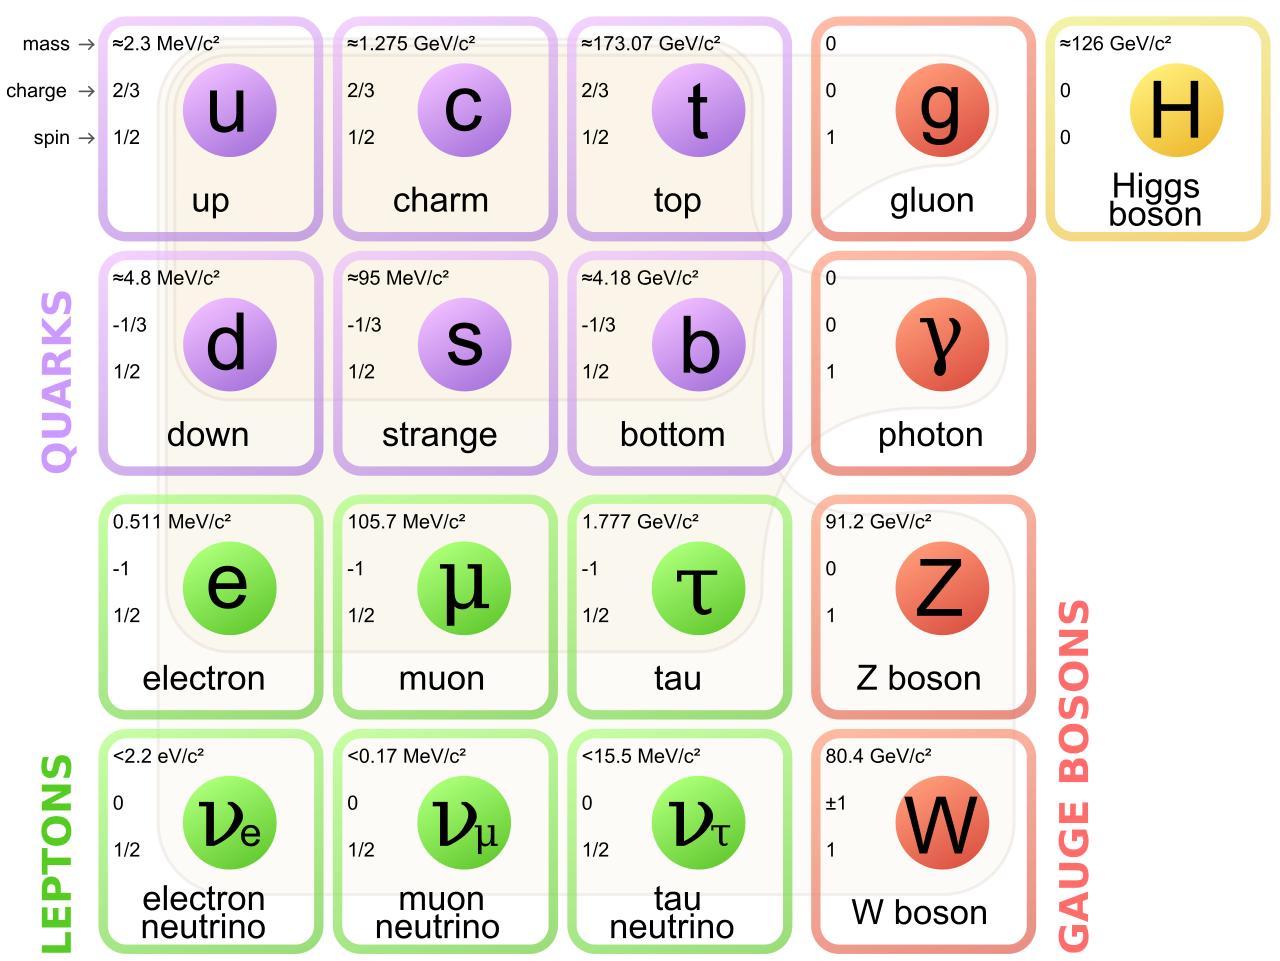
\includegraphics[width=0.8\linewidth]{../figures/images/standard_model.png}
\end{figure}
}

\addframe{Charmonium}{
Resonances formed by a $\qcharm\aqcharm$ pair: $\jpsi, \; \psip, \; \psipp, \; \ldots$
\additem{$\psip$ and $\psipp$ originally interpreted as excited states of $\jpsi$}
\additem{Evidence of mixed-states suggests more complicated picture}

\begin{figure}
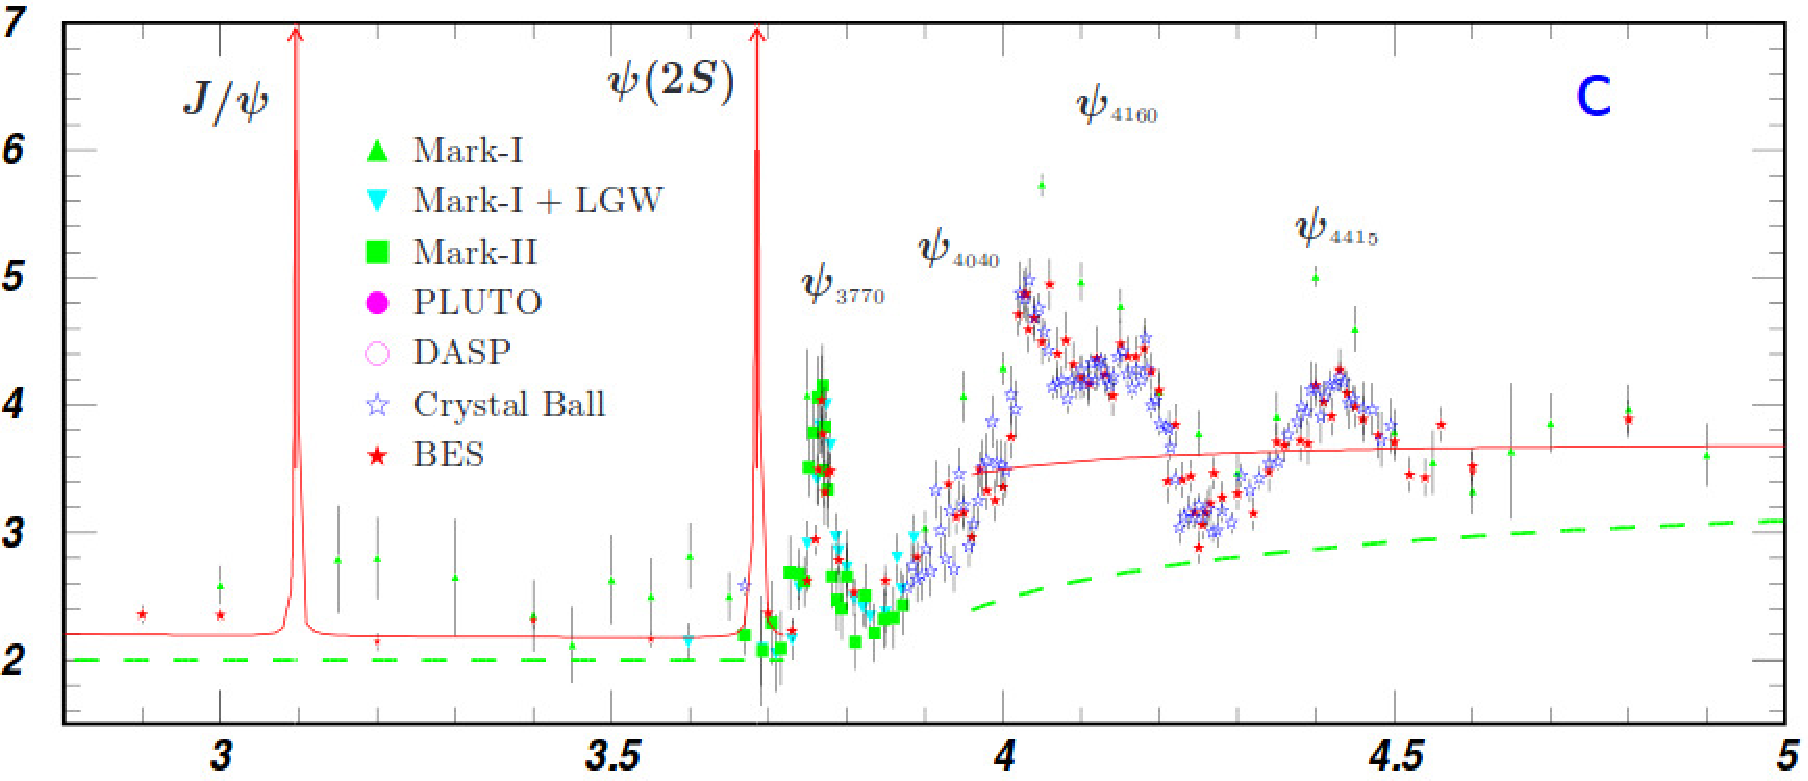
\includegraphics[width=\linewidth]{../figures/images/R_scan.pdf}
\end{figure}
}

\addframe{OZI Rule}{

\vspace{-1.0cm}

\begin{columns}

\column{.5\textwidth} % Left column and width
\addcenter{\textbf{$\psip$}}

\vspace{-0.5cm}

\begin{figure}
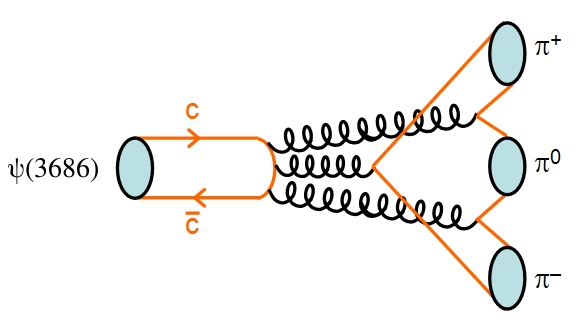
\includegraphics[width=\linewidth]{../figures/images/OZI_psip.png}
\end{figure}

\begin{itemize}
\item Requires three gluons for decay 

\item{Very narrow decay width
\additem{$\Gamma_{\psip} = \SI{0.286}{\MeV}$}}

\end{itemize}

\column{.5\textwidth} % Right column and width
\addcenter{\textbf{$\psipp$}}

\vspace{-0.3cm}

\begin{figure}
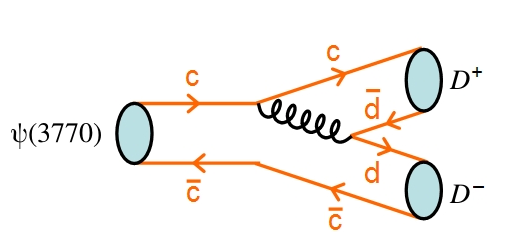
\includegraphics[width=\linewidth]{../figures/images/OZI_psipp.png}
\end{figure}

\vspace{0.35cm}

\begin{itemize}

\item Decays via open charm ($\DDbar$)

\item {Much wider decay width
\additem{$\Gamma_{\psipp} = \SI{27.5}{\MeV}$}}

\end{itemize}

\end{columns}

\vspace{0.3cm}

\addcenter{Addition of $\DDbar$ decays introduces drastically different behavior!}
}

\sectionframe{Accelerator and Detector}
% Show pictures of Beijing map and campus, if possible 

\addframe{Institute of High Energy Physics (IHEP)}{
\vspace{-0.3cm}

\addcenter{BESIII is hosted at the IHEP Campus located in Beijing, China}

\vspace{-0.3cm}

\begin{figure}
\includegraphics[width=\linewidth]{../figures/images/BESIII_layout.jpg}
\end{figure}
}

\addframe{Accelerator - Beijing Electron-Positron Collider II (BEPCII)}{

\begin{enumerate}

\item{Create positrons by firing electrons into stationary material
\additem{Generates high energy $\gamma$s which interact with material to form $\ee$}}

\item{Separate newly created positrons magnetically}

\item{Accelerate positrons in linear accelerator and feed into storage ring}

\item{Accelerate electrons and feed into the oppositely circulating ring
\additem{Electrons readily available, so extraction from photons unnecessary}}

\item{Focus each beam using magnets along storage rings until collision}

\end{enumerate}

\begin{figure}
\includegraphics[width=0.42\linewidth]{../figures/images/accelerator.jpg}
\hspace{1.5cm}
\includegraphics[width=0.42\linewidth]{../figures/images/storage_ring.jpg}
\end{figure}

}

\addframe{Detector - Beijing Spectrometer III (BESIII)}{
Collision of beams tuned to occur at central point of detector
\additem{Beams angled during collision to improve integrated luminosity}

\vspace{-0.3cm}

\begin{columns}

\column{.5\textwidth} % Left column and width

Four main subdetector systems:
\begin{itemize}
\item Main Drift Chamber
\item Time-of-Flight
\item Electromagnetic Calorimeter
\item Muon Identifier 
\end{itemize}

\vspace{-0.3cm}

\begin{figure}
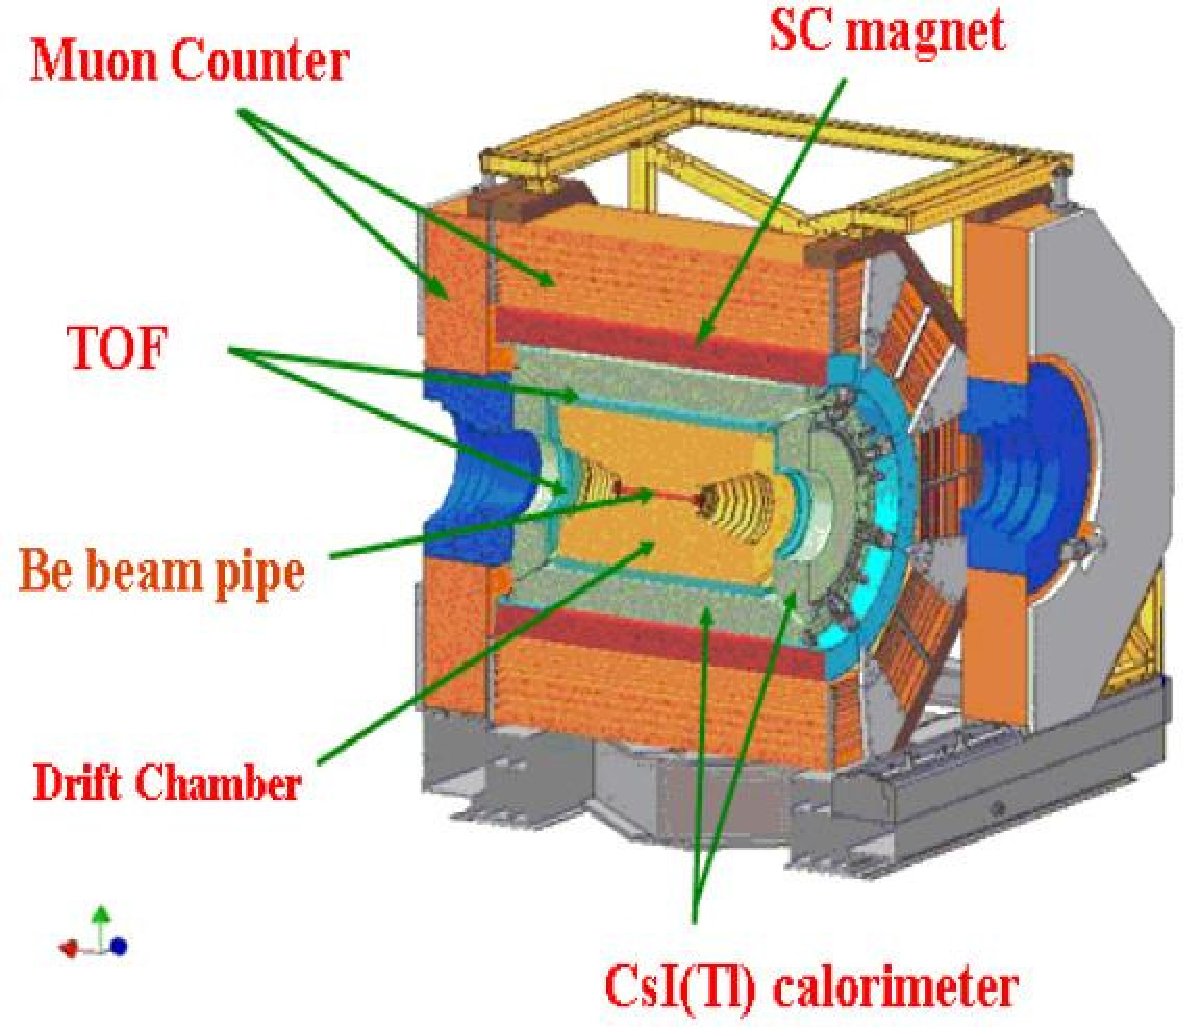
\includegraphics[width=0.85\linewidth]{../figures/images/detector.jpg}
\end{figure}

\column{.5\textwidth} % Right column and width

\begin{figure}
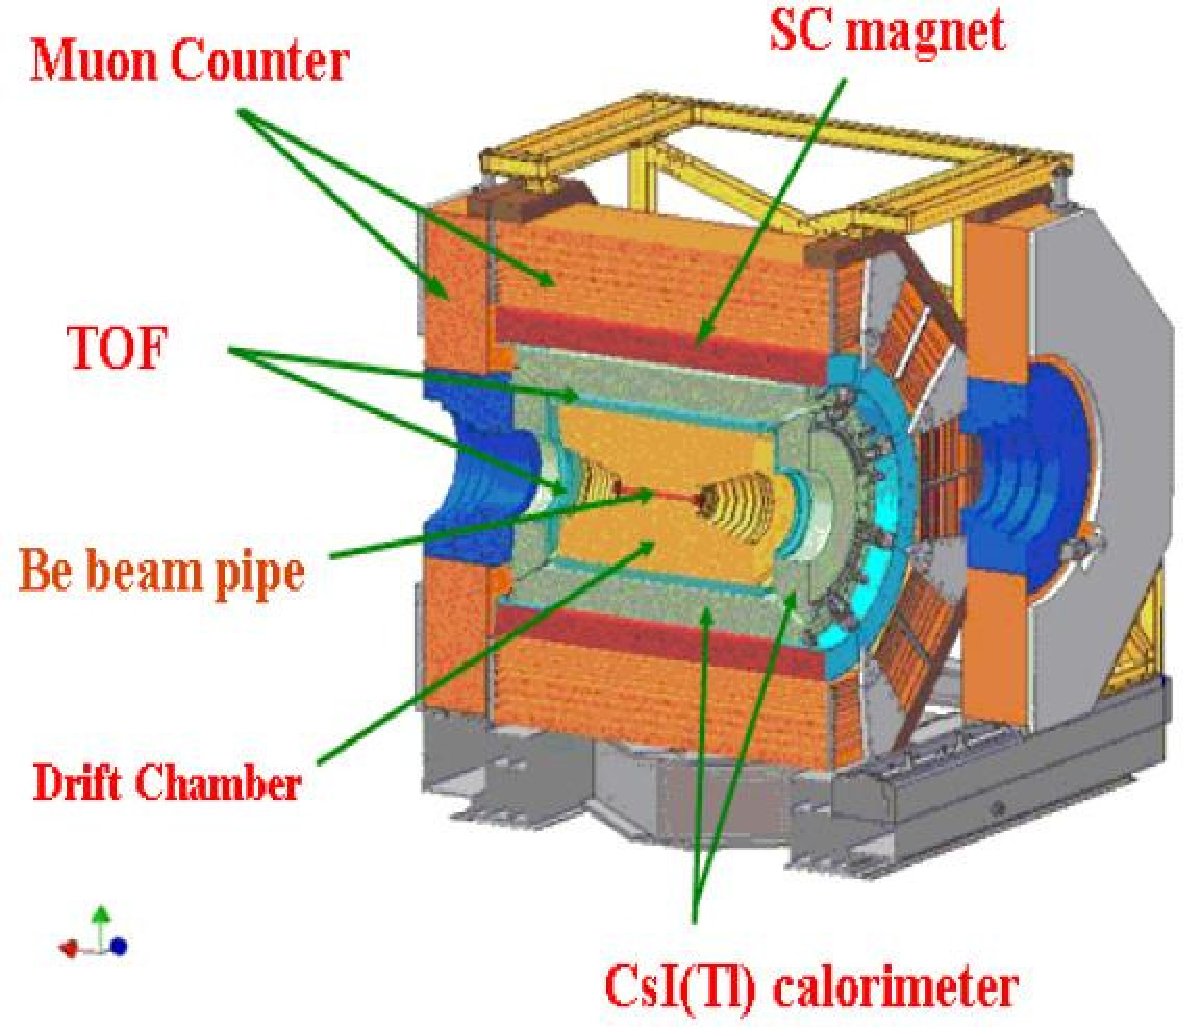
\includegraphics[width=\linewidth]{../figures/images/detector.pdf}
\end{figure}

\end{columns}

}

\addframe{Main Drift Chamber (MDC)}{
\vspace{-0.8cm}
\begin{columns}

\column{.55\textwidth} % Left column and width

\additem{Reconstruct charged tracks from interactions with sense wires (hits)
\additem{Wires surrounded by ionizable gas}
\additem{Initial ionization due to particle triggers avalanche of electrons}
\additem{High electric field near wires draws in released electrons to measure energy deposited}
}

\additem{Determine properties of particle from curvature in magnetic field
\additem{Radius determines momentum}
\additem{Direction determines charge}
}

\additem{Energy deposition rate ($\tdEdx$) helps determine particle candidate}


\column{.5\textwidth} % Right column and width

\addcenter{
BESIII Event Display

\begin{figure}
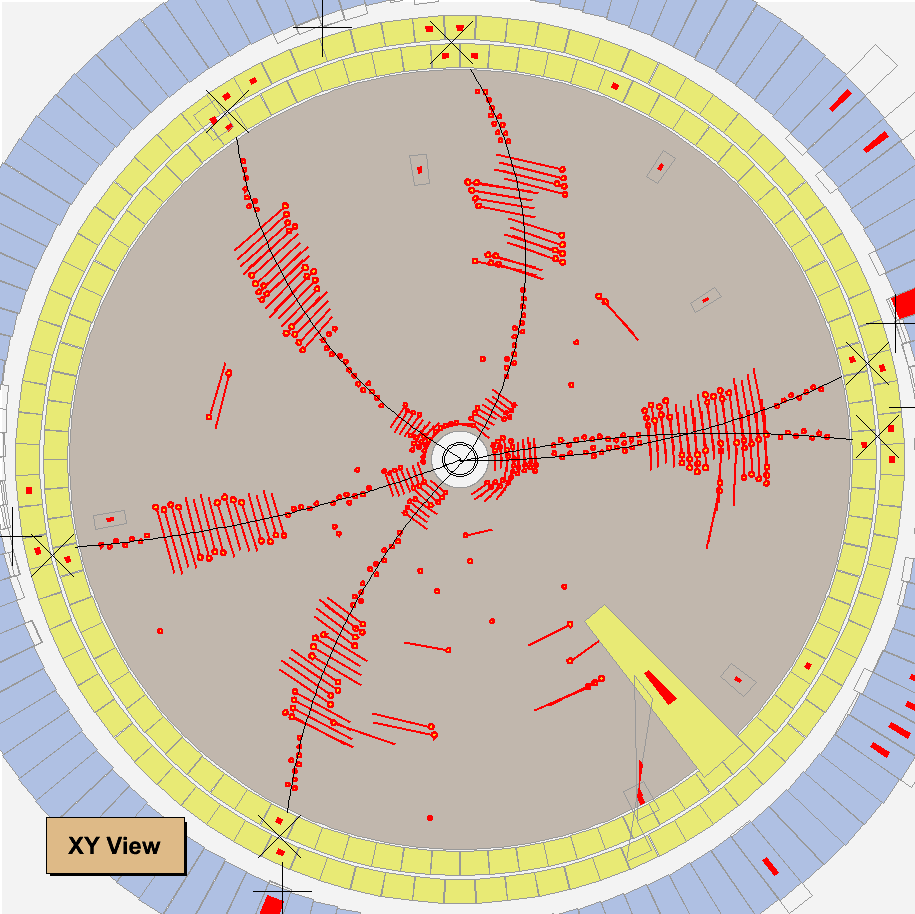
\includegraphics[width=\linewidth]{../figures/images/BESVis.png}
\end{figure}
}

\end{columns}
}

\addframe{Time-of-Flight (ToF)}{

\additem{Measure particle velocity using travel time after initial collision 
\additem{Scintillator bands located at \SIlist{0.81;0.86}{\m} from interaction point}
\additem{Attached to photomultiplier tubes to measure light output}
}

\additem{Helps distinguish between $\Kpm$ and $\pipm$ candidates at lower momenta
\additem{Combined with $\tdEdx$ measurements in MDC to set particle hypothesis}
}

\vspace{-0.6cm}

\begin{columns}

\column{0.5\textwidth} % Left column and width
\addcenter{MDC Measurements}

\vspace{-0.6cm}

\begin{figure}
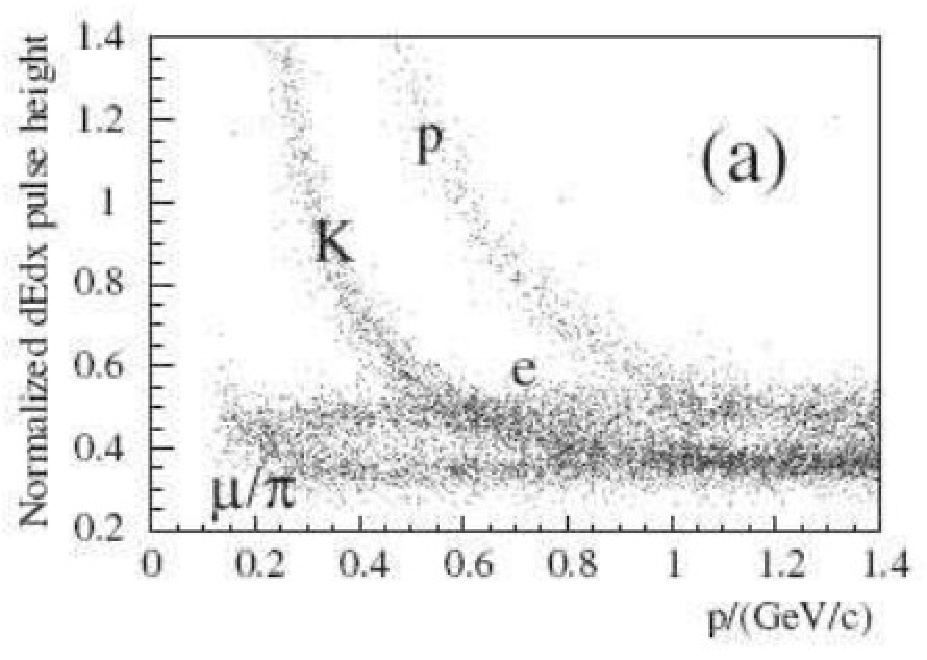
\includegraphics[width=\linewidth]{../figures/images/dEdx.pdf}
\end{figure}


\column{0.5\textwidth} % Right column and width
\addcenter{ToF Measurements}

\vspace{-0.6cm}

\begin{figure}
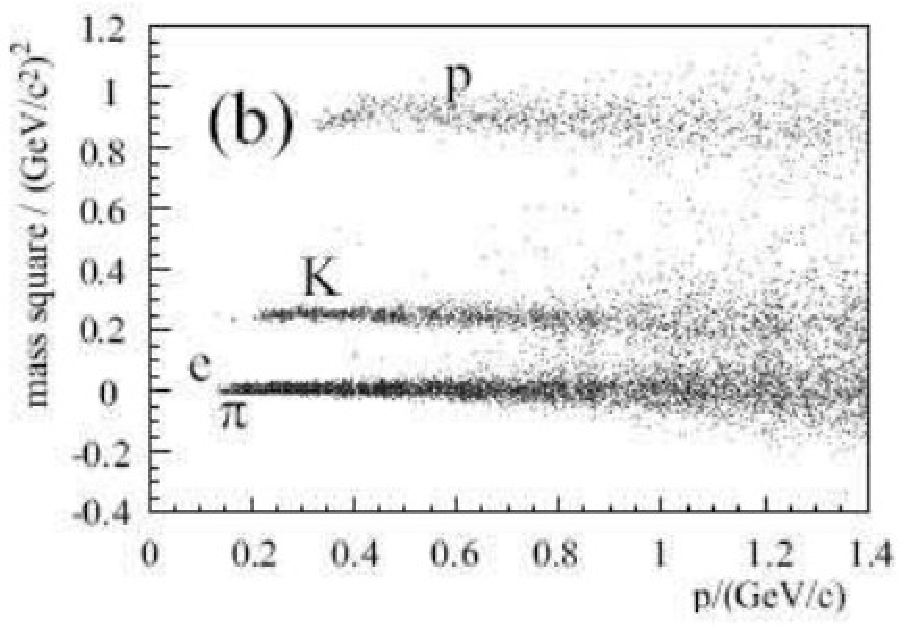
\includegraphics[width=\linewidth]{../figures/images/ToF.pdf}
\end{figure}

\end{columns}
}

\addframe{Electromagnetic Calorimeter (EMC)}{
\additem{Measure energy deposited by electron and photon tracks
\additem{Other particles are generally relativistic and thereby minimum ionizing
\additem{These deposit relatively constant energy, independent of momenta}
}
\additem{Use CsI(Tl) crystals attached to photodiodes to measure energy
\additem{Energy lost primarily in gaps of arrangement or out the back of crystals}
}
}
\additem{Allows reconstruction of purely neutral decays, such as $\piO \rightarrow \photon\photon$}

\begin{figure}
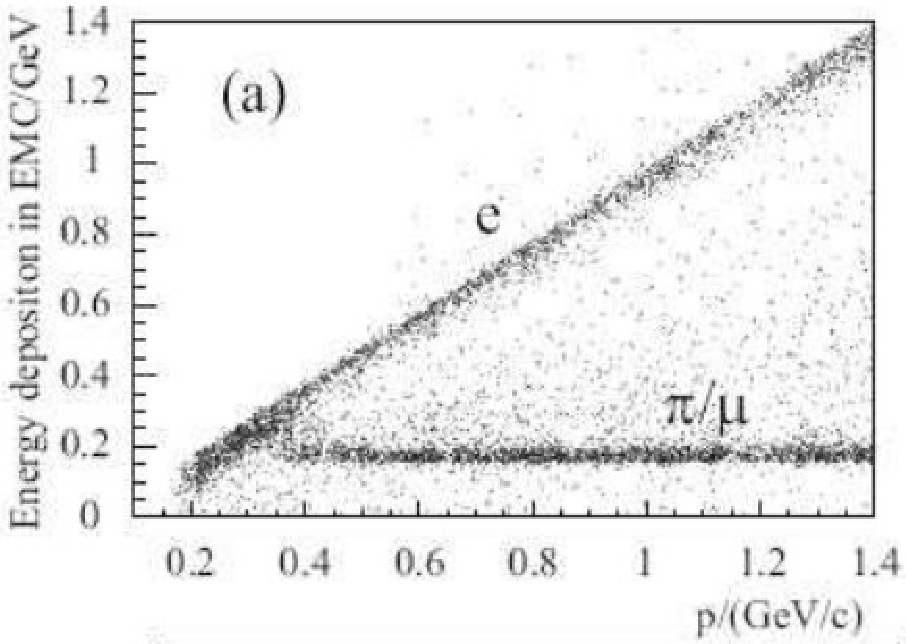
\includegraphics[width=0.5\linewidth]{../figures/images/EMC.pdf}
\end{figure}
}

\addframe{Muon Identifier (MUC)}{
\additem{Identify tracks traversing through multiple layers as muons
\additem{Most particle types will be stopped before reaching the MUC
\additem{Electrons susceptible to Bremsstrahlung radiation}
\additem{Kaons and pions susceptible to strong interactions}
}
\additem{Requires muons with $p > \SI{0.4}{\GeV}$ for appropriate curvature}
}
}

\addframe{Triggering System}{
Collisions filtered unless passing event reconstruction criteria
}


\sectionframe{Analysis Software}{
% Show images of event display and... generic code? I dont know

\addframe{Monte Carlo Generation}{
Describe process and usage of MC samples
}

\addframe{Monte Carlo Generators}{
Describe usage of KKMC

Describe usage of BesEvtGen

Describe usage of Babayaga
}

\addframe{$D$-Tagging}{
Describe process and usage of $D$-Tagging
}

\addframe{Selection Cuts}{
Show cuts on $\pipm, \Kpm, \piO, \Ks$
}


\sectionframe{Measurement of the $\DDbar$ Cross Section}
% Show images of derivation formulas, energy measurements, fitting plots, cross sections, and systematics

\addframe{Procedure}{
Derive theoretical model used to describe cross section

List data samples used for measurement

Determine $\Ecm$ and $\lum$ for each data point

Identify signal and background components

Measure efficiency of reconstruction

Combine everything to determine cross section

Assess systematic uncertainties
}

\addframe{Derivation of $\xsecpsipptoDDbar$ - Part I}{
Show derivation of cross section
}

\addframe{Derivation of $\xsecpsipptoDDbar$ - Part II}{
Show derivation of cross section
}

\addframe{Derivation of $\xsecpsipptoDDbar$ - Part III}{
Show derivation of cross section
}

\addframe{Form Factors}{
Explain form factor choices and describe necessary modifications
}

\addframe{Data Samples}{
Show scan data and describe usage $\psipp$, $R$-scan, and $XYZ$-scan samples
}

\addframe{Center-of-Mass Energy}{
Describe measurement and correction process
}

\addframe{Luminosity}{
Describe measurement process
}

\addframe{Monte Carlo Generation}{
List included MC samples and explain KKMC modification
}

\addframe{Signal Determination}{
Describe process of 2D fitting to $\DeltaE$ and $\mbc$

Show example results plot near $\psipp$
}

\addframe{Efficiency Correction}{
Describe process of averaging efficiency over all decay modes
}

\addframe{$\sCP$ Violation Correction}{
Quickly list process of correcting for $\sCP$
}

\addframe{Cross Section Fitting}{
Describe procedure of obtaining $\psipp$ parameters
}

\addframe{Exponential Results}{
Show Exponential results
}

\addframe{Vector Dominance Model Results}{
Show VDM results
}

\addframe{Systematic Uncertainties}{
Describe process of measuring systematics
}

\addframe{Systematics}{
Luminosity

$\pipm / \Kpm$ Tracking

$\piO$ Tracking

$\Ks$ Tracking

Single Tag Fitting

PDG Branching Fractions

Meson Radii
}

\addframe{Negligible Systematics}{
MC Iteration

MC ISR Generation

Intermediate Resonances
}

\addframe{Model Dependent Systematic}{
Form Factor assumption
}

\addframe{Final Results}{
Show final results with systematics

Compare to KEDR and PDG
}


\sectionframe{Measurement of the $\NonDDbar$ Branching Fraction}
% Show images of data counts, extrapolations, $\DDbar$ corrections

\addframe{Procedure}{
Event Selection

Hadron Cut Methods

Signal Counting Fits

MC Background Subtraction

Efficiency Extrapolation

$\DDbar$ Multiplicity Correction

Examination of Results for $\psipp$ Data

Background Investigation

Examination of Results for Scan Data
}

\addframe{Data Samples}{
Show 3650 Data Sets

Mention energy measurement
}

\addframe{Event Selection}{
Charged Track Selection

Neutral Track Selection

Background Rejection
}

\addframe{Hadronic Selection}{
Show SHAD, LHAD, and THAD cut tables
}

\addframe{Signal Counting}{
Show signal counting fits for data
}

\addframe{Background Subtraction}{
List MC samples considered (and note those excluded)

Relate to total number of hadrons found for future extrapolation
}

\addframe{Efficiency Extrapolation}{
Repeat procedure for new continuum data

Extrapolate efficiency based on $\Ecm$

Show extrapolation plots for SHAD, LHAD, and THAD
}

\addframe{Procedure for $\psipp$ Data}{
Repeat procedure for $\psipp$ data

Introduction of new backgrounds and $\DDbar$ component
}

\addframe{$\DDbar$ Correction}{
Create multiplicity distributions from single-tag events

Obtain correction factors for R1 and R2 separately

Example plots for $\DO$ and $\Dp$ of R1
}

\addframe{Reconstruction Efficiencies}{
Show different backgrounds for SHAD

Describe correction used for $\ypsip$ events

Point out cross sections used by Derrick for $\psipp$ data
}

\addframe{Initial Results - $\psipp$ Data}{
Show cross section / branching fractions

Point out likely high values due to $\psip$ shape
}

\addframe{Background Investigation - Part I}{
Describe alternate estimation for $\psip$ events

Show branching fraction results with estimation
}

\addframe{Background Investigation - Part II}{
Describe alternate estimation ignoring $\psip$ events

Show branching fraction results with estimation
}

\addframe{Procedure for Scan Data}{
Using best information available from $\psipp$ results

Show hadronic cross section over region
}

\addframe{Results for Scan Data}{
Show $\nonDDbar$ cross section over region

Show $\nonDDbar$ branching fraction over region
}


\sectionframe{Conclusion}

\addframe{Conclusion}{
Show overview of measurements for $\DDbar$ cross section and $\nonDDbar$ branching fraction

List results of parameters for $\psipp$

List branching fraction range for $\nonDDbar$
}

\end{document} 
